\pdfoutput=1
\pdfminorversion=4

\documentclass[preprint]{elsarticle}
\usepackage[utf8]{inputenc}

%packages
\usepackage[margin=1in]{geometry}

\usepackage[hyphens]{url}
\biboptions{sort&compress, square, comma}
\usepackage[breaklinks=true, linkcolor=blue, citecolor=blue, colorlinks=true]{hyperref}

\usepackage{graphicx}
\usepackage{caption}
\usepackage{subcaption}

\usepackage{booktabs}

\usepackage[version=3]{mhchem} % Formula subscripts using \ce{}, e.g., \ce{H2SO4}
\usepackage{latexsym,amsmath,amssymb}

\usepackage{mathtools}
\usepackage{tablefootnote}

%better printing of numbers
\usepackage[T1]{fontenc}
\usepackage[english]{babel}
\usepackage{csquotes}
\usepackage{textcomp}

\usepackage{algorithm}
\usepackage[noend]{algpseudocode}
\makeatletter
\let\OldStatex\Statex
\renewcommand{\Statex}[1][3]{%
  \setlength\@tempdima{\algorithmicindent}%
  \OldStatex\hskip\dimexpr#1\@tempdima\relax}

\usepackage[binary-units]{siunitx}
\sisetup{group-separator={,},
     detect-all,
     binary-units,
     list-units = single,
     range-units = single,
     range-phrase = --, 
     per-mode = symbol-or-fraction,
     separate-uncertainty = true,
     list-final-separator = {, and }
%    scientific-notation = fixed
}
\DeclareSIUnit\atm{atm}

% Add [disable] option to quickly remove any
\usepackage[textsize=small,textwidth=2.25cm]{todonotes}

%custom commands
\newcommand{\NA}{---}
\newcommand{\centercell}[1]{\multicolumn{1}{c}{#1}}
\newcommand{\centermulti}[2]{\multicolumn{#2}{c}{#1}}
\newcommand{\head}[1]{\centercell{\bfseries#1}}
\newcommand{\headmulti}[2]{\centermulti{\bfseries#1}{#2}}

\journal{36th International Symposium on Combustion}

\begin{document}
\begin{frontmatter}

\title{An investigation of GPU-accelerated chemical kinetic integration methods}

\author[uconn]{Nicholas~J.\ Curtis}
\author[osu]{Kyle~E.\ Niemeyer}
\author[uconn]{Chih-Jen Sung\corref{cor1}}
\ead{cjsung@engr.uconn.edu}

% addresses
\address[uconn]{Department of Mechanical Engineering\\
  University of Connecticut, Storrs, CT, 06269, USA}
\address[osu]{School of Mechanical, Industrial, and Manufacturing Engineering\\
  Oregon State University, Corvallis, OR 97331, USA}
  
\cortext[cor1]{Corresponding author}

\begin{abstract}
A fifth-order implicit Runge--Kutta method and two fourth-order exponential integration methods equipped with Krylov subspace approximations were implemented for the GPU and paired with the analytical chemical kinetic Jacobian code \texttt{pyJac}.
The performance of each was compared to the commonly used CPU-based implicit integrator \texttt{CVODE}.
The implicit Runge--Kutta method performed up to eight times faster on a single GPU than \texttt{CVODE} on a single six-core CPU for an \ce{H2}\slash \ce{CO} model, and ran competitively with \texttt{CVODE} for the GRI-Mech.\ 3 model.
The exponential integration techniques performed less efficiently for all cases.
The main limiter of GPU integrator performance was identified as thread divergence, and techniques to mitigate this issue were discussed.
A novel shared memory caching strategy for the GPU was developed and shown to provide a \SIrange{5}{10}{\percent} performance increase to all GPU-based integrators.
Additionally, an issue affecting storage of the chemical kinetic Jacobian in per-thread local memory was identified.
Work-around methods were discussed and the resulting balance between chemical kinetic mechanism size and independent ODEs solved per kernel launch was explored.
Finally, future research directions were identified based on the current state-of-the-art of stiff chemical kinetic integration on the GPU.
\end{abstract}

\begin{keyword}
 Chemical kinetics \sep Stiff chemistry \sep SIMD \sep GPU
\end{keyword}

\end{frontmatter}
\pagebreak

%%%%%%%%%%%%%%%%%%%%%%%%%%%%%%%%%%%%%%%%%%%%
\section{Introduction}
\label{sec:Intro}
%%%%%%%%%%%%%%%%%%%%%%%%%%%%%%%%%%%%%%%%%%%%

The need for accurate chemical kinetic models in predictive reacting-flow simulations has driven the development of detailed oxidation models for hydrocarbon fuels relevant to transportation and energy generation applications.
At the same time, growing understanding of the hydrocarbon oxidation process resulted in orders of magnitude increases in model size and complexity.
For instance, a recently developed model for 2-methylalkanes, relevant for jet and diesel fuel surrogates, consists of over 7000 species and 30000 reactions~\cite{Sarathy:2011kx} while a recent detailed gasoline surrogate mechanism contains over 1500 species and 6000 reactions~\cite{Mehl:2011jn}.
Furthermore, kinetic models for large hydrocarbon fuels tend to exhibit chemical stiffness requiring implicit integration algorithms, the solution cost of which scale at best quadratically---and at worst cubically---with the number of species in a mechanism~\cite{Lu:2009gh}.

Consequently, a number of techniques have been developed to accelerate chemical kinetics integration.
As Lu and Law reviewed more extensively~\cite{Lu:2009gh}, these methods can be roughly categorized into three classes: skeletal reduction and removal of unimportant species and reactions~\cite{Lu:2005,Pepiot-Desjardins:2008,Niemeyer:2010bt,Niemeyer:2014,Curtis:2015aa}, time-scale analysis~\cite{qssa,pe_approx1,pe_approx2} and dimensional reduction~\cite{Lam:1988wc,Maas:1992aa,Lu:2001ve}, and tabulation\slash interpolation of expensive terms~\cite{Pope:1997wu,Christo1996}.
In addition to these cost-reduction methods, significant work has been directed towards improvements of the integration algorithms themselves.

Reactive-flow modeling codes commonly rely on high-order implicit integration techniques to solve the stiff governing equations posed by chemical kinetics models.
These methods require repeated evaluation and factorization of the chemical kinetic Jacobian matrix in order to solve the associated non-linear algebraic equations through iterations of linear system solutions, the cost of which scales quadratically and cubically, respectively, with the number of species in a mechanism.
However, significant cost savings in the Jacobian evaluation can be realized through the use of an analytic formulation, rather than the typical evaluation via finite difference approximations.
This approach eliminates numerous chemical source term evaluations, and for a sparse Jacobian (e.g. formulated in terms of species concentrations) the cost of evaluation drops to a linear dependence on the number of species in the mechanism~\cite{Lu:2009gh}.
Several analytical Jacobian matrix codes have been developed~\cite{Safta:2011vn,Youssefi:2011tm,Bisetti:2012jw,Perini:2012gy,Dijkmans:2014bb}, but the recently released \texttt{pyJac} software~\cite{Niemeyer:2015im,Niemeyer:2015ws} is currently the only open-source analytical chemical kinetic Jacobian tool capable of generating code for single-instruction multiple-data (SIMD) processor types such as graphics processing units (GPUs), as well as handling newer pressure-dependent reaction formulations (e.g., pressure-log, Chebyshev).

Further acceleration of chemical kinetic integration techniques focused on improving the integration itself, via development of new algorithms and use of high-performance hardware accelerators such as GPUs and other similar SIMD devices.
Central processing unit (CPU) clock speeds increased regularly over the past few decades---commonly known as Moore's Law---however, power consumption and heat dissipation issues slowed this trend recently.
While multi-core parallelism somewhat increased CPU performance, recently SIMD processors gained popularity as a low cost, low power consumption, and massively parallel high-performance computing alternative.
GPUs were originally developed for graphics\slash video processing applications and consist of hundreds to thousands of separate cores, compared to the tens of cores found on typical CPUs.
The SIMD parallelism model differs from a traditional CPU-based multi-threading model, with small per-core memory caches and acceleration resulting from executing the same instruction over multiple data.
For more details, we refer the reader to several works that discussed these differences in depth~\cite{Cruz:2011gc,Brodtkorb:2013hn,Niemeyer:2014hn}.

A number of studies in recent years explored the use high-performance SIMD devices to accelerate (turbulent) reacting-flow simulations.
Spafford et al.~\cite{Spafford:2010aa} investigated using GPUs to accelerate a turbulent combustion direct numerical simulation code, demonstrating a sub-order of magnitude speedup in evaluating the species production rates on the GPU.
Shi et al.~\cite{Shi:2011aa} used a GPU to evaluate species rates and factorize the Jacobian for the integration of independent kinetics systems, showing order-of-magnitude or greater speedups for large kinetic models.
Niemeyer et al.~\cite{Niemeyer:2011aa} implemented an explicit fourth-order Runge--Kutta integrator for the GPU, and found a speedup of nearly two orders of magnitude with a non-stiff hydrogen mechanism.
Shi et al.~\cite{Shi:2012aa} implemented a stabilized explicit solver and paired it with a CPU-based implicit solver that handled integration of the most-stiff chemistry cells in a three-dimensional premixed diesel engine simulation, demonstrating an overall speedup of \numrange{2}{3}$\times$.
Le et al.~\cite{Le2013596} implemented a GPU version of two high-order shock-capturing reacting flow codes, and found a \numrange{30}{50}$\times$ speedup over the baseline.
Stone et al.~\cite{Stone:2013aa} implemented the implicit VODE~\cite{brown1989vode} solver for the GPU and achieved an order of magnitude speed-up over the baseline CPU version.
Additionally, they showed that the implicit VODE algorithm exhibited significant thread divergence, as expected due to its complicated program flow (compared to an explicit integration scheme).
Furthermore, Stone et al.~\cite{Stone:2013aa} showed that, for numbers of independent ODE systems greater than $\sim$\SI{e3}, using individual GPU threads to handle independent chemical kinetic ODEs offered greater performance over using a block of GPU threads to cooperatively solve a single ODE~\cite{Stone:2013aa}.
Niemeyer et al.~\cite{Niemeyer:2014aa} demonstrated an order-of-magnitude speedup for an implementation of a stabilized explicit second-order Runge--Kutta--Chebyshev algorithm over a multi-core CPU implementation of VODE for moderately stiff chemical kinetics.
They also investigated levels of thread divergence due to differing integrator time step sizes, and found it negatively impacts overall performance for dissimilar ODE initial conditions in a thread-block.
Sewerin et al.~\cite{Sewerin20151375} implemented a three-stage\slash fifth-order implicit Runge--Kutta method~\cite{wanner1991solving} on a one-block per ODE basis, and found a $1.8\times$ slowdown at best compared to the same on a single eight-core CPU.

While increasing numbers of studies have explored GPU acceleration of chemical kinetics, there remains a clear need to find or develop integration algorithms simultaneously suited for the SIMD parallelism of GPUs and similar accelerators and capable of handling stiffness.
In this work we will investigate GPU implementations of several semi-implicit and implicit integration techniques, as compared to their CPU counterparts and a baseline CPU VODE implementation~\cite{Hindmarsh:2005hg}.
Several previous works~\cite{Perini20141180,McNenly2015581} suggested so-called matrix-free methods---which do not require direct factorization of the Jacobian, but instead use an iterative process to approximate the action of the factorized Jacobian on a vector---as potential improvements to the expensive linear-system solver required in standard implicit methods.
Further, as demonstrated by Hochbruck et al.~\cite{Hochbruck:1997} the convergence of the matrix-exponential, $exp(\tau A)v$ using Krylov subspace approximation is faster than that of the corresponding Krylov methods for the solution of linear equations $(I - \tau A)x = v$.
Methods of this type, called explicit exponential integration methods have previously been explored for applications in stiff chemical systems~\cite{Bisetti:2012jw,falati2011integration} and were found to be stable for time-steps greatly exceeding the stability bound.
In addition, their explicit nature makes them potentially much better suited for SIMD acceleration due an expected reduction of thread-divergence as compared to implicit methods.
Furthermore, the three-stage, fifth-order implicit Runge--Kutta algorithm~\cite{wanner1991solving} investigated by Sewerin et al.~\cite{Sewerin20151375} will be studied to determine the impact of increasing chemical stiffness on the algorithm and the performance benefits of using an analytical Jacobian matrix.

%%%%%%%%%%%%%%%%%%%%%%%%%%%%%%%%%%%%%%%%%%%%
\section{Methodology}
\label{sec:Method}
%%%%%%%%%%%%%%%%%%%%%%%%%%%%%%%%%%%%%%%%%%%%

In this section, we discuss details of the algorithms implemented for the GPU along with third-party software used.
The generation of testing conditions will be discussed briefly, and a shared memory caching algorithm will be outlined.

%%%%%%%%%%%%%%%%%%%%%%%%%%%%%%%%%%%%%%%%%%%%
\subsection{Integration techniques}

We investigated GPU implementations of three integration methods in this work, comparing them against equivalent CPU versions and a CPU-only implicit algorithm.
While we describe important details or changes here, full descriptions of all algorithms may be found in the cited sources.
The aforementioned \texttt{pyJac} software~\cite{Niemeyer:2015im} provided both chemical source term and analytical Jacobian subroutines for CPU- and GPU-based algorithms.
For validation and performance assessments of \texttt{pyJac}, we direct readers to our previous work~\cite{Niemeyer:2015ws}.

First, we used the \texttt{CVODE} solver~\cite{Hindmarsh:2005hg} to provide the baseline performance of a typical CPU-based high-order implicit integration technique.
In addition, we implemented CPU versions of the methods under investigation for direct comparison to the high-order implicit technique.
These include the three-stage/fifth-order implicit Runge--Kutta algorithm~\cite{wanner1991solving}, called \texttt{Radau-IIA} here; the fourth-order exponential Rosenbrock-like method \texttt{exp4} of Hochbruck et al.~\cite{Hochbruck:1998}; and the newer fourth-order exponential Rosenbrock method~\cite{Hockbruck:2009}, called \texttt{exprb43} here.
For the exponential methods, we used the method of rational approximants~\cite{gallopoulos:1992} paired with the Carath\'edothy--Fej\'er method~\cite{trefethen:2006} to approximate the action of the matrix exponential on a vector, as suggested by Bisetti~\cite{Bisetti:2012jw}.
This technique relied on the external \texttt{FFTW3} library~\cite{frigo2005design}.
However, unlike the approach of Bisetti, we developed a custom routine based on the algorithm presented by Stewart~\cite{stewart:1998} to perform the LU decomposition of the Hessenberg matrix resulting from the Arnoldi iteration.
To ensure high performance of CPU-based methods, the Intel \texttt{MKL} library version 11.1.3 handled linear algebra (i.e., BLAS/LAPACK) operations.
Next, we implemented GPU versions of the \texttt{Radau-IIA}, \texttt{exp4}, and \texttt{exprb43} methods; these follow the same descriptions as the CPU versions, but required specialized implementations of several BLAS and LAPACK methods, mostly related to LU factorization (or Hessenberg LU factorization for the exponential integrators).
All GPU routines were developed using the NVIDIA CUDA framework~\cite{Buck:2008aa,NVIDIA:2015aa}.
Finally, the adaptive timestepping procedures of all integrators used absolute and relative tolerances of \SI{1e-15} and \SI{1e-8}, respectively, throughout the work, and the exponential integrators used a rational approximant type of $\left(10,10\right)$ as suggested by Bisetti~\cite{Bisetti:2012jw}.

%%%%%%%%%%%%%%%%%%%%%%%%%%%%%%%%%%%%%%%%%%%%
\subsection{Testing conditions}

In order to validate and measure the performance of the integrators for realistic conditions, a database of thermochemical conditions covering a wide range of temperatures and species mass fractions was generated using a previously developed stochastic partially stirred reactor (PaSR) code~\cite{Niemeyer:2015ws}.
Table~\ref{T:mechanisms} describes the two chemical kinetic mechanisms selected to span the range of model sizes typically used in high-fidelity simulations.
The PaSR simulations were performed at the conditions listed in Table~\ref{T:pasr_parameters} for ten residence times to reach a statistical steady state; Niemeyer et al.~\cite{Niemeyer:2015ws} describe the PaSR simulation process in greater detail, which follows approaches used by others~\cite{Chen:1997ta,Pope:1997wu,Ren:2004fz,Ren:2014cd}.

\label{S:pasr}
\begin{table}[htb]
\centering
\begin{tabular}{@{}l l l l@{}}
\toprule
Fuel species & \# of species & \# of reactions & Reference \\
\midrule
\ce{H2}\slash \ce{CO} & 13 & 27 &~\cite{Burke:2011fh} \\
\ce{CH4} & 53 & 325 &~\cite{smith_gri-mech_30} \\
\bottomrule
\end{tabular}
\caption{
Summary of chemical kinetic models used as benchmark test cases.
}
\label{T:mechanisms}
\end{table}

\begin{table}[htb]
\centering
\begin{tabular}{@{}l l l @{}}
\toprule
Parameter & \ce{H2}\slash air & \ce{CH4}\slash air \\
\midrule
$\phi$ & \multicolumn{2}{c}{1} \\
$T$ & \multicolumn{2}{c}{\SIlist{400;600;800}{\kelvin}} \\
$p$ & \multicolumn{2}{c}{\SIlist{1;10;25}{\atm}} \\
$N_p$ & \multicolumn{2}{c}{100} \\
$\tau_{\text{res}}$ & \SI{10}{\milli\second} & \SI{5}{\milli\second} \\
$\tau_{\text{mix}}$ & \SI{1}{\milli\second} & \SI{1}{\milli\second} \\
$\tau_{\text{pair}}$ & \SI{1}{\milli\second} & \SI{1}{\milli\second} \\
\bottomrule
\end{tabular}
\caption{
PaSR parameters used for hydrogen\slash air, methane\slash air, and ethylene\slash air premixed combustion cases, where $\phi$ indicates equivalence ratio, $T$ is temperature, $p$ is pressure, $N_p$ is the number of particles, $\tau_{\text{res}}$ is the residence time, $\tau_{\text{mix}}$ is the mixing time, and $\tau_{\text{pair}}$ is the pairing time.
}
\label{T:pasr_parameters}
\end{table}

%%%%%%%%%%%%%%%%%%%%%%%%%%%%%%%%%%%%%%%%%%%%
\subsection{Shared memory caching}

\todo[inline]{This section may need a bit more of an introduction, because shared memory seems to come out of nowhere.}
When formulated in a single-ODE-per-thread basis, GPU-based algorithms must split a relatively small cache memory (typically \SI{64}{\kilo\byte}) between all threads in the blocks resident on a streaming multiprocessor.
Most versions of the CUDA compute standards further segregate this cache into a L1 cache, and memory shared between threads in a block and allow the user to control whether the L1 cache or the shared memory will be larger.\todo{something wrong with this sentence}
In our study, we found using a larger L1 cache always performs better, which may be expected for the per-thread approach where register spilling and global memory accesses are unavoidable.
This leaves a significant portion of the cache ($\sim$\SI{16}{\kilo\byte}) as shared memory, but the small number of available memory locations per thread---two to four doubles---poses challenges to using this fast memory efficiently in the integration algorithm itself.
However, the evaluations of the chemical source terms and analytical Jacobian often use species concentrations and reaction rates during consecutive operations, presenting an opportunity to exploit the available shared memory.
Algorithm~\ref{A:shared_mem_caching} describes an algorithm to use this available shared memory for the reaction rate subroutine. 
Similar algorithms were developed for the species rate and Jacobian evaluation routines, using species rates and reaction rates\slash species concentrations as the cacheable variables, respectively.
As this algorithm generates the source code for the various subroutines, it introduces no computational or memory overhead related to determining the caching structure during runtime.
Although this represents a relatively simple improvement, its use can achieve reasonable performance benefits, as will be seen in Sec.~\ref{S:smem}.

% I assume "hardware" was a typo extra there
\begin{algorithm}[htb]
\caption{Shared memory caching during evaluation of reaction rates.}
\begin{algorithmic}[0]
%  \State {Initialize the cached species concentration set $C_{0} = \varnothing$; the maximum set size is $C_{max}$}
%  \For {$R_i$ in reactions}
%    \State Let $S_i$ be the set of participating species in $R_i$
%    \State Let $P_{i,j}$ be the number of consecutive reactions starting from $R_{i + 1}$ 
%    \Statex that each species $S_j$ in $R_i$ participates in
%    \State Let $L_{i,j}$ be the number of reactions since $C_{i,j}$ has participated directly in a reaction
%    \State Sort $S_{i}$ in descending order by $P_{i,j}$ and store in $S_{i}^{\prime}$
%    \For {$S_{i,j}$ in $S_{i}^{\prime}$}
%      \If{$\|C_i\| < C_{max}$}
%	\State Add $S_{i,j}$ to $C_i$
%      \ElsIf{$\max \left(L_{i}\right) \geq 2$ and $P_{i,j}$ > 1}
%	  \State Set $k$ such that $L_{i,k} = \max\left(L_{i}\right)$
%	  \State Replace $C_{i,k}$ with $S_{i,j}$, and remove $S_{i,j}$ from $S_{i}^{\prime}$
%      \EndIf
%    \EndFor
%    \For {$S_{i,j}$ in $S_{i}^{\prime}$}
%      \If{$\|S_{i}^{\prime}\| > 0$ and $\|C_i\| < C_{max}$}
%	\State Add $S_{i,j}$ to $C_i$
%      \EndIf
%    \EndFor
%    \State Compute reaction rate $i$ using values in $C_i$ where appropriate.
%  \EndFor
  \State {Initialize the cached species concentration set $C_{0} = \varnothing$; the maximum set size is $C_{max}$}
  \For {$r_i$ in reactions $R$}
    \State Let $S_i$ be the set of participating species in $r_i$
    \State Let $P_{i,j}$ be the number of consecutive reactions starting from $r_{i + 1}$ 
    \Statex in which each species $s_{i,j}$ of $S_i$ participates
    \State Let $L_{i,j}$ be the number of reactions since $s_{i,j}$ participated directly in a reaction
    \State Sort $s_{i,j}$ in descending order by $P_{i,j}$ and store in $S_{i}^{\prime}$
    \For {$s_{i,j}$ in $S_{i}^{\prime}$}
      \If{$\|C_i\| < C_{max}$}
	\State Add $s_{i,j}$ to $C_i$
      \ElsIf{$\max \left(L_{i}\right) \geq 2$ and $P_{i,j}$ > 1}
	  \State Set $k$ such that $L_{i,k} = \max\left(L_{i}\right)$
	  \State Replace $C_{i,k}$ with $s_{i,j}$, and remove $s_{i,j}$ from $S_{i}^{\prime}$
      \EndIf
    \EndFor
    \For {$s_{i,j}$ in $S_{i}^{\prime}$}
      \If{$\|S_{i}^{\prime}\| > 0$ and $\|C_i\| < C_{max}$}
	\State Add $s_{i,j}$ to $C_i$
      \EndIf
    \EndFor
    \State Compute reaction rate of $i$ using values in $C_i$ where appropriate.
  \EndFor
\end{algorithmic}
\label{A:shared_mem_caching}
\todo[inline]{I'm a little confused by some of the notation; not sure what $C_{i,j}$ is, and then you drop the second subscript in a few lines. Same with $C_i$, where before you used $C_{i,j}$. I made some changes, namely using lower case for items and upper case for sets. But, I'm still confused about the first use of $C_i$.}
\end{algorithm}

%%%%%%%%%%%%%%%%%%%%%%%%%%%%%%%%%%%%%%%%%%%%
\section{Results and discussion}
%%%%%%%%%%%%%%%%%%%%%%%%%%%%%%%%%%%%%%%%%%%%

\subsection{Performance}

The performance of the integrators was tested on the PaSR conditions described in Section~\ref{S:pasr} for two different global integration timesteps representative of those used in large eddy and Reynolds-averaged Navier--Stokes simulations: $\delta t = \SI{1e-6}{\s}$ and $\delta t = \SI{1e-4}{\s}$, respectively.
Furthermore, the use of a larger global timestep induces additional stiffness for a given mechanism and enables evaluation of integrator performance at varying stiffness levels.
All reported runtimes were averaged over five runs, each run starting from the same set of PaSR conditions.
The uncertainties in runtimes were not plotted as they could not be represented in a way that did not detract from the comprehensibility of the figures, but were fairly minimal except for small numbers of ODEs where the runtimes were very short.
All CPU integrators were compiled using \texttt{gcc 4.4.7}, and were run in parallel on a six-core Intel Xeon X5650 using \texttt{OpenMP}, while all GPU integrators were compiled with \texttt{nvcc 7.0.27} and run on a single NVIDIA Tesla C2075.
The open source \texttt{pyJac} code~\cite{Niemeyer:2015im,Niemeyer:2015ws} was used for rate and analytical Jacobian evaluation for both the CPU and GPU.

\begin{figure}[htb]
  \centering
  \begin{subfigure}{0.49\textwidth}
      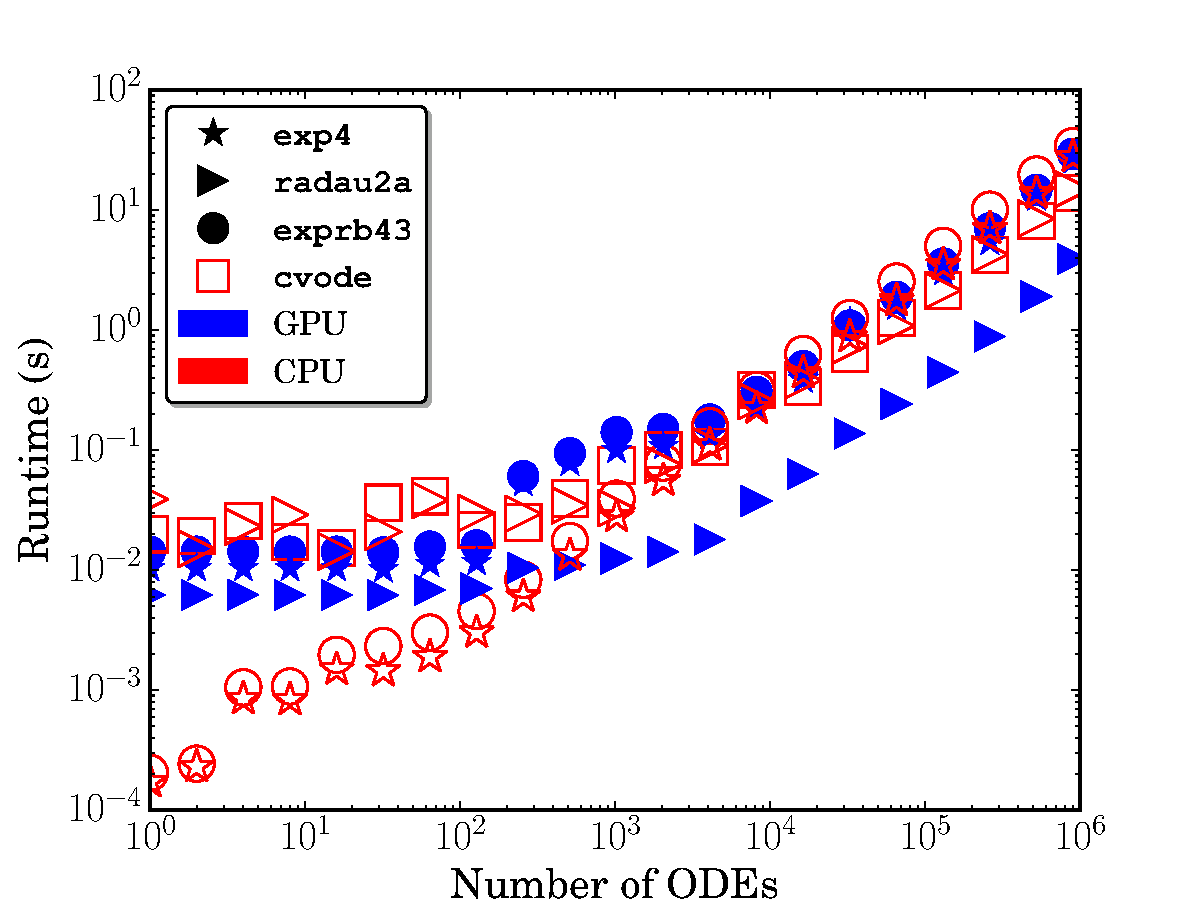
\includegraphics[width=\linewidth]{H2_1e-06_cpuvsgpu.pdf}
      \caption{$\delta t = \SI{1e-6}{\sec}$}   
  \end{subfigure}
  %\hfill
  \begin{subfigure}{0.49\textwidth}
      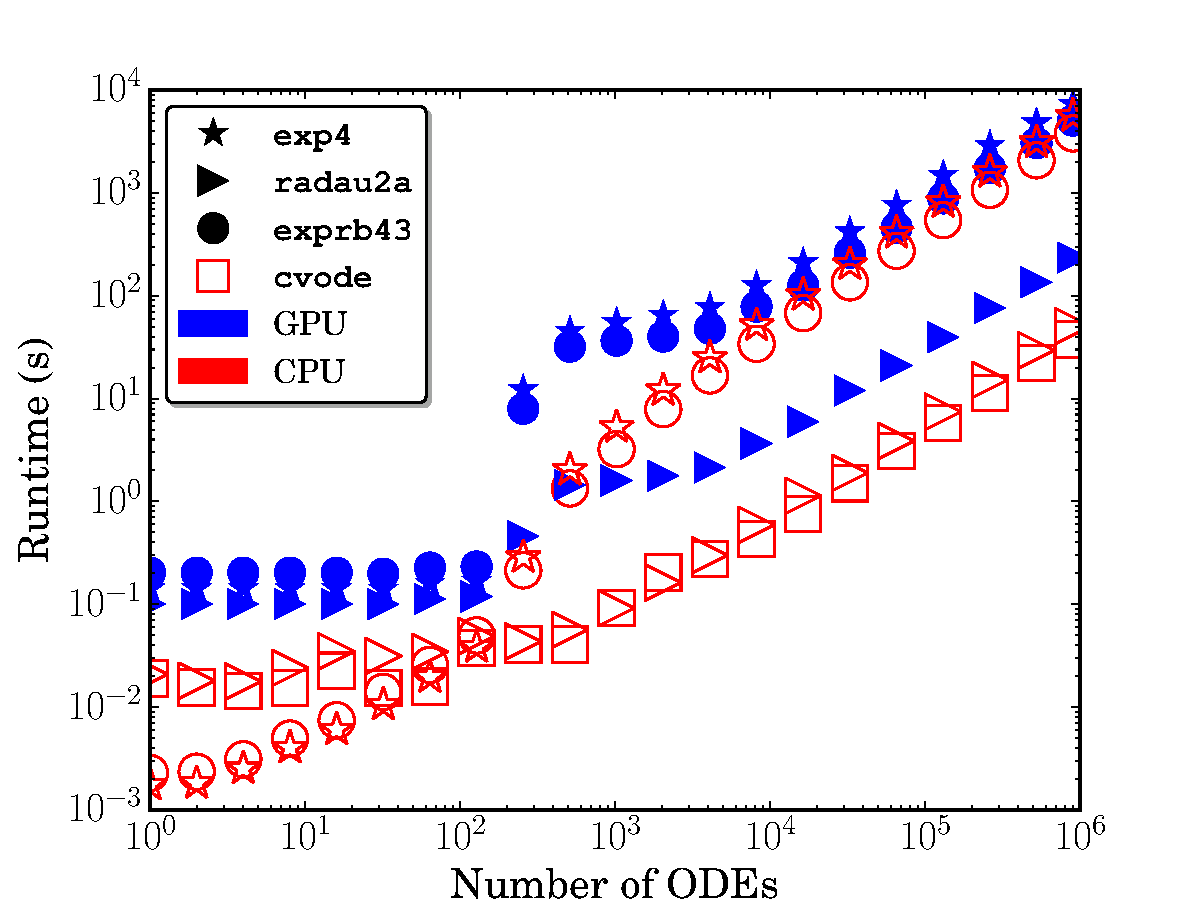
\includegraphics[width=\linewidth]{H2_1e-04_cpuvsgpu.pdf}
      \caption{$\delta t = \SI{1e-4}{\sec}$}
  \end{subfigure}
  \caption{Average runtimes of the integrators for the \ce{H2} mechanism at two different global timesteps. 
  CPU versions were run in parallel on six cores.}
  \label{F:H2_perf}
\end{figure}

Figure~\ref{F:H2_perf} shows the runtimes of the integrators for the \ce{H2} mechanism.
The CPU \texttt{Radau-IIa} integrator had roughly equivalent performance compared to \texttt{CVODE} for the smaller global timestep, and was only slightly slower \texttt{CVODE} for the larger timestep.
The GPU \texttt{Radau-IIa} integrator was at best $8.41\times$ faster than \texttt{CVODE}, and was on average $5.39\pm1.35\times$ faster for the smaller timestep (counting only runtimes for more than 1024 ODEs, where the GPU becomes fully utilized).
Using the the larger timestep negatively impacted the performance of the GPU \texttt{Radau-IIa} integrator and it was at best $2.69\times$ faster, and $1.78\pm0.81\times$ slower on average.
Both the CPU and GPU versions of the exponential integrators were reasonably similar in performance to the CPU implicit integrators, and at the smaller timestep the GPU versions generally outperformed their CPU counterparts.
Although the \texttt{exprb43} and \texttt{exp4} algorithms each only require three exponential matrix function approximations, \texttt{exprb43} is more expensive for a single step due to the extra chemical source term evaluations\slash matrix multiplications, and the higher-order phi function requirement.
As such, the CPU \texttt{exprb43} integrator generally is outperformed by the relatively more simple \texttt{exp4} integrator for the smaller timestep.
However, for the larger timestep with higher stiffness the expected order reduction~\cite{Bisetti:2012jw} of the \texttt{exp4} integrator makes it less efficient than \texttt{exprb43}.

\begin{figure}[htb]
  \centering
  \begin{subfigure}{0.49\textwidth}
      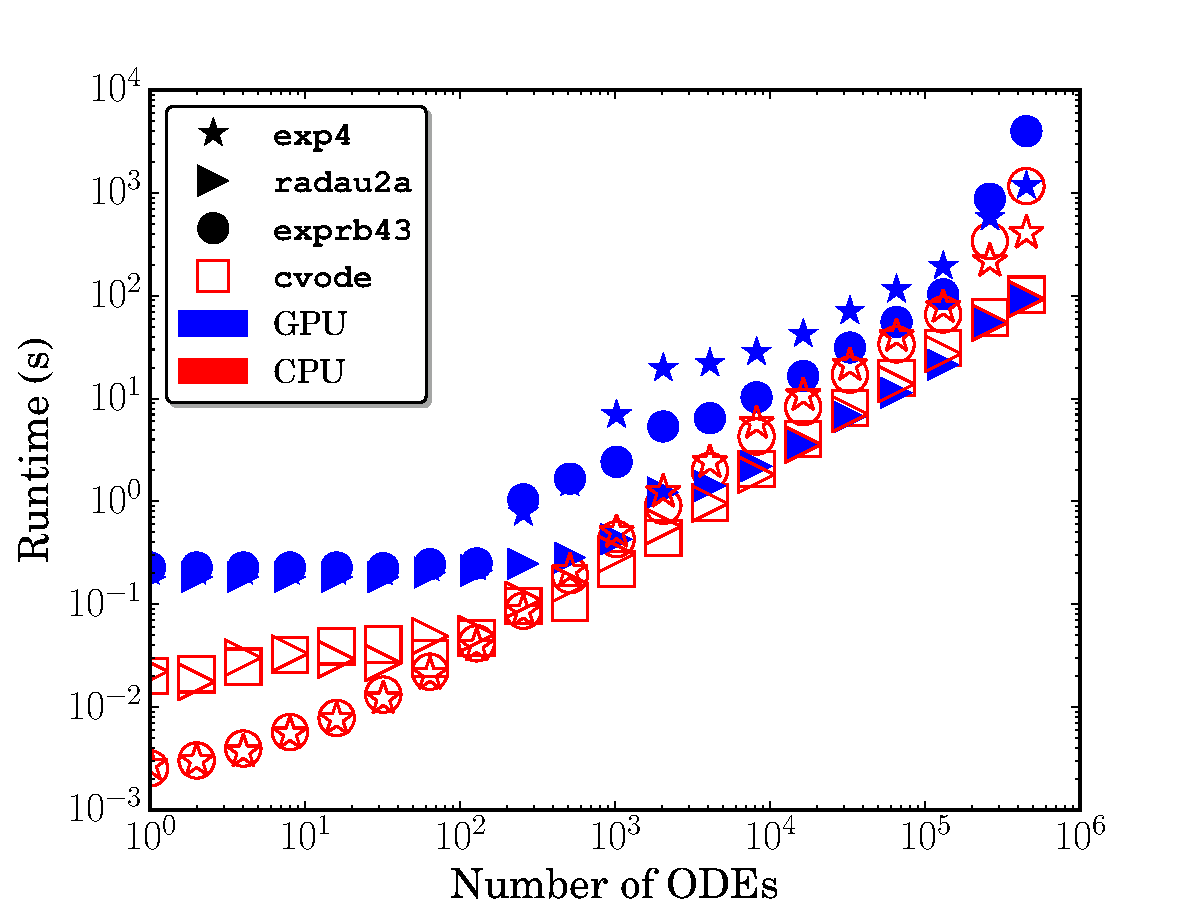
\includegraphics[width=\linewidth]{GRI_1e-06_cpuvsgpu.pdf}
      \caption{$\delta t = \SI{1e-6}{\sec}$}
  \end{subfigure}
  %\hfill
  \begin{subfigure}{0.49\textwidth}
      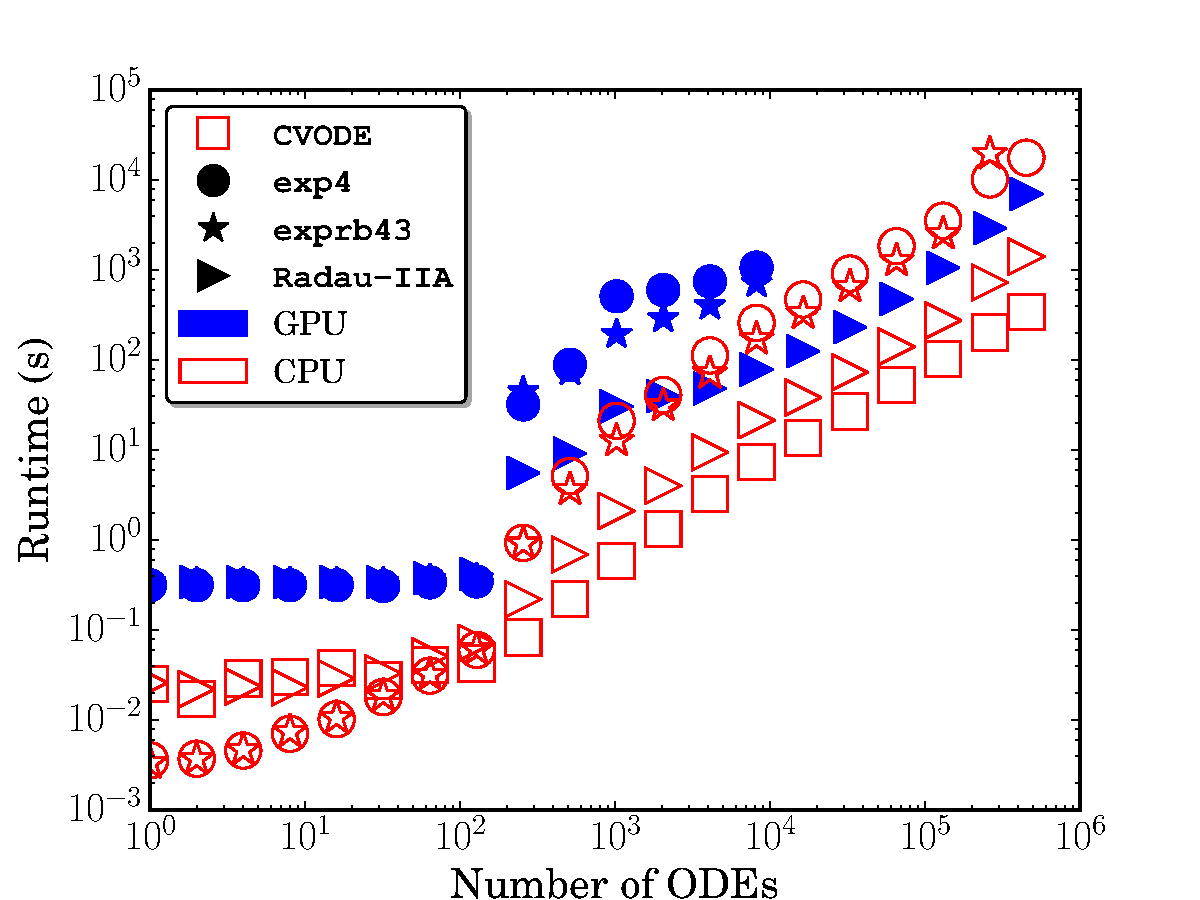
\includegraphics[width=\linewidth]{GRI_1e-04_cpuvsgpu.pdf}
      \caption{$\delta t = \SI{1e-4}{\sec}$}
  \end{subfigure}
  \caption{Average runtimes of the integrators for the GRI Mech.~3.0 mechanism at two different global timesteps. 
  CPU versions were run in parallel on six cores.
  Some of the longer running exponential integration cases were omitted.}
  \label{F:GRI_perf}
\end{figure}

Figure~\ref{F:GRI_perf} shows the runtime of the integrators for the GRI mechanism.
The GPU \texttt{Radau-IIa} integrator often outperforms the CPU version and \texttt{CVODE} for the smaller timestep; it is at best $1.46\times$ faster, and is on average $1.13\pm0.63\times$ slower then \texttt{CVODE}.
For the larger timestep the performance of the GPU \texttt{Radau-IIa} integrator is again negatively impacted, dropping to a best case of $8.63\times$ slower, and $14.18\pm6.64\times$ slower on average.

Two different major factors affect the performance of the GPU integration algorithms, chemical stiffness and thread divergence.
The performance of the CPU \texttt{Radau-IIa} integrator is almost identical to that of \texttt{CVODE} except for the stiffest case, the GRI mechanism with the larger timestep.
This difference may be due to the adaptive order nature of the \texttt{CVODE} algorithm, or potentially due to its maturity and years of optimization.
However, this effect is fairly minor and should not cause the order of magnitude decrease in relative performance between the GPU \texttt{Radau-IIa} integrator and \texttt{CVODE} observed when switching to the larger timestep.
To investigate this further, we adopted a similar quantification of thread divergence to that of Niemeyer et al.~\cite{Niemeyer:2014aa}:
\begin{equation}
	D = \frac{\sum_{i=1}^{32}{d_i}}{32 \max_{i \in 32} d_i}
	\label{eqn:divergence}
\end{equation}
where $d_i$ is the number of internal integrator timesteps taken to reach the global timestep by thread $i$ in a warp.
If a warp experiences no thread divergence due to differing internal integration timesteps this measure will be one, however if the number of internal integration timesteps is highly unbalanced in a warp this measure will tend to zero.

\begin{figure}[htb]
  \centering
  \begin{subfigure}{0.49\textwidth}
      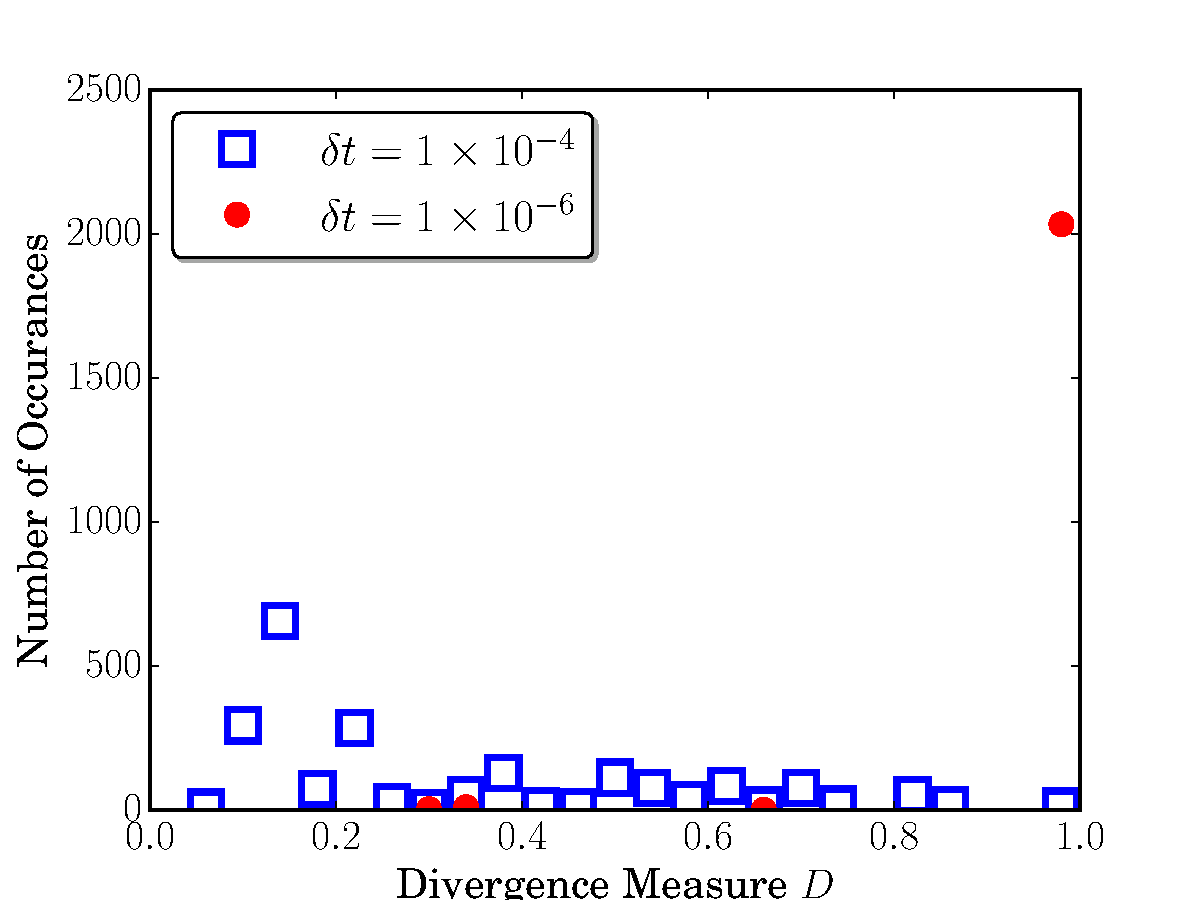
\includegraphics[width=\linewidth]{H2_radau2a_div.pdf}
      \caption{\ce{H2} mechanism}
  \end{subfigure}
  %\hfill
  \begin{subfigure}{0.49\textwidth}
      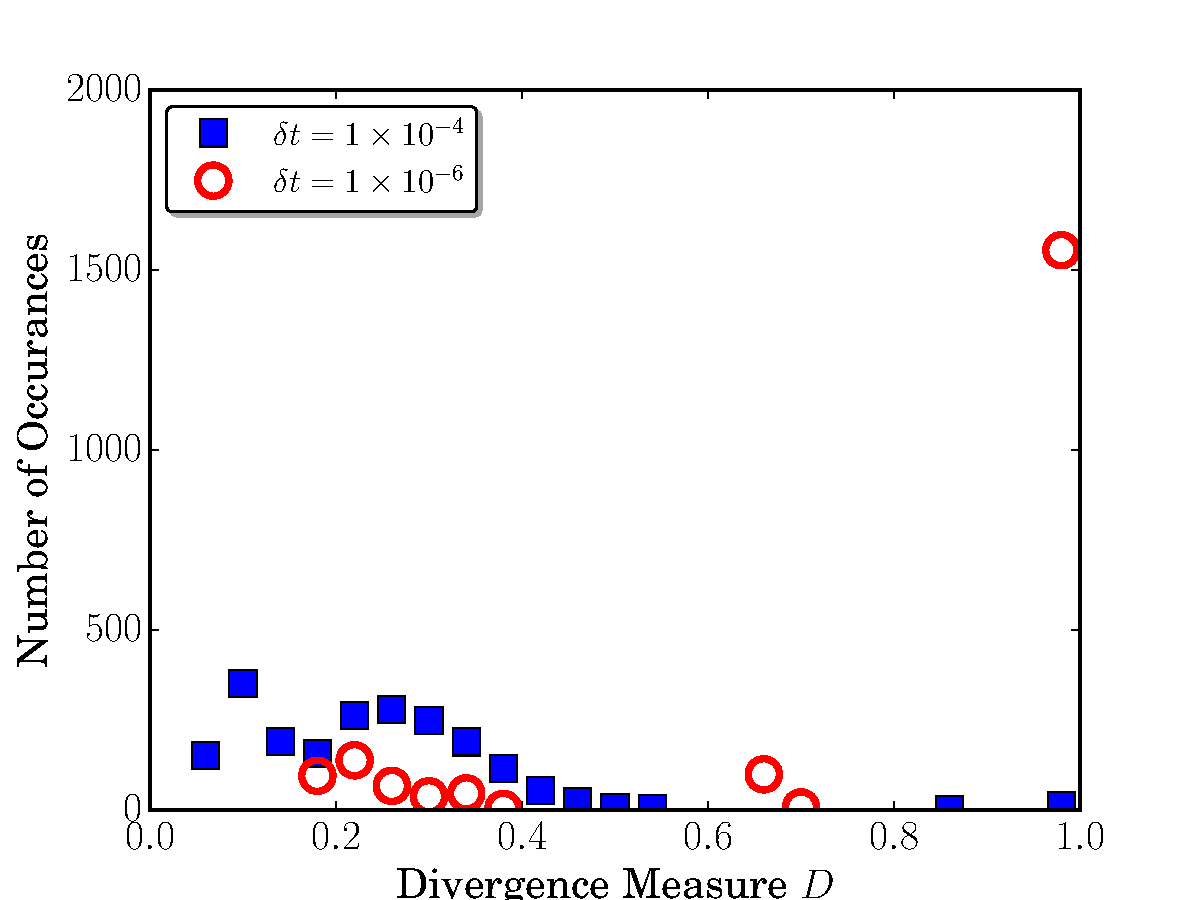
\includegraphics[width=\linewidth]{CH4_radau2a_div.pdf}
      \caption{GRI mechanism}
  \end{subfigure}
  \caption{Thread divergence measure of the \texttt{Radau-IIa} solver for both mechanisms and timesteps.}
  \label{F:divergence}
\end{figure}

Figure~\ref{F:divergence} shows the distribution of the divergence measure of the \texttt{Radau-IIa} solver for both timesteps and mechanisms when run on \num{65536} ODEs (\num{2048} warps).
For both mechanisms, the number of warps where large thread divergence occurs increases drastically with an increasing timestep.
This implies that thread divergence, rather than purely chemical stiffness, is the main performance limiter for the GPU \texttt{Radau-IIa} integrator.
Further, the relative performance difference of the GPU \texttt{Radau-IIa} solver between the \ce{H2} mechanism and the GRI mechanism at the smaller timestep is likely partially due to the increased thread divergence between the mechanisms.
Therefore, our future work will be aimed at development of strategies to reduce thread divergence.
Potential solutions include adoption of an ODE per-block approach, re-ordering of ODEs to increase similarity of chemical stiffness inside a warp or timestep synchronization between threads in a warp.
\todo[inline]{If time, run Radau studies with 100 consecutive $10^{-6}$ timesteps for the $10^{-4}$ global timestep case to see effect on performance and emphasize this point}

Figure~\ref{F:GRI_perf} also shows that the performance of the CPU exponential integrators is similar to that of the implicit CPU integrators for the smaller timestep.
As the exponential integrators must only factorize a much smaller Hessenberg matrix rather than the entire Jacobian---as in the implicit integrators---significant savings in factorization can potentially be achieved with larger mechanism sizes.
However, as the stiffness is increased, e.g., as in the large timestep case, the stability characteristics of the implicit integrators again makes them more favorable.
Thus the exponential integrators may be more efficient than the implicit integrators for moderately stiff systems (e.g., with small timesteps, or low tolerances) of larger chemical mechanisms.
Although not shown in Fig.~\ref{F:divergence}, the exponential integrators experienced significant thread divergence in all cases, and thus would also likely benefit from the thread divergence reduction techniques discussed above.

\subsection{Effect of shared memory caching}
\label{S:smem}

The effectiveness of the shared memory caching scheme was evaluated in several cases by comparing the mean runtime of the integrators using rate and analytical Jacobian subroutines generated with and without the caching algorithm enabled.
A typical speedup of $\sim\SI{5}{\percent}$ was seen for the smaller global timestep cases, while a $\sim\SI{10}{\percent}$ speedup was observed for the larger timestep cases.
This difference is due to increase in chemical source term and Jacobian evaluations required for the larger timestep cases.
In certain cases for the GRI mechanism, even larger speedups were observed, e.g. a \SI{24.4}{\percent} speedup with \texttt{exp4} for \num{131072} ODEs and the \SI{e-6}{\second} timestep, and a \SI{13.2}{\percent} speedup with \text{Radau-IIa} for \SI{32768} ODEs and the \SI{e-4}{\second} timestep.


\subsection{Limitations of per-thread local memory for implicit GPU integration}

During work on this paper, a significant but under discussed issue with the use of implicit and semi-implicit integrators on the GPU came to light.
Namely, the size of the Jacobian places severe restrictions on either the maximum allowable mechanism size, or the total number of independent chemical-kinetic ODEs that can be solved concurrently.
For instance, the \texttt{Radau-IIA} solver requires storage of the Jacobian, as well as a LU factorized and a complex LU factorized matrix of the same size.
Similarly, the exponential integrators require storage of the Jacobian, the Hessenberg matrix and vector subspace resulting from the Arnoldi process and the corresponding exponential of the Hessenberg matrix.
While the Hessenberg matrix, exponential Hessenberg matrix, and vector subspaces can be smaller than the full Jacobian (e.g., by limiting the maximum Kyrlov subspace size), for the sake of simplicity in this analysis we shall assume they are full sized.
This implies that the storage requirements per ODE solved concurrently scales as $\mathcal{O}\left(3 \times N_s^2\right)$ for the \texttt{Radau-IIA} solver and as $\mathcal{O}\left(4 \times N_s^2\right)$ for the exponential solvers, where $N_s$ is the number of species in the mechanism.

One method of storing these matrices (and other integrator variables) is in per-thread local memory (which resides in global device memory).
This is advantageous from a programming standpoint, as it ensures coalesced memory access and simplifies indexing.
In CUDA however, all threads are limited to a maximum of \SI{512}{\kilo\byte} local memory, or \num{64000} double precision floating point numbers.
This limits the maximum mechanism size to relatively small numbers, as seen in Table~\ref{T:size_limits}, for GPU solvers implemented on a per-thread basis.
In this study, even the USC mechanism \ce{C2H4}~\cite{Wang:2007} with only 111 species caused the GPU to run out of local thread memory for all three GPU integrators.

Instead, the Jacobian and associated matrices can be pre-allocated in global memory, and thus the total global memory is split between all ODEs to be solved in a given kernel launch.
In this work, a Tesla C2075 GPU was used, and recent GPU-based chemical kinetic integration studies have used similar models~\cite{Shi:2011aa,Niemeyer:2011aa,Shi:2012aa,Le2013596,Stone:2013aa,Niemeyer:2014aa}
For a \SI{6}{\giga\byte} global memory size and \num{e6} independent ODEs, this works out to just 750 doubles available per concurrent ODE.
Even assuming a more reasonable \SI{e5} ODEs, or low \SI{e4} ODEs per kernel launch, each concurrent ODE is limited to just \num{7500} and \num{75000} doubles correspondingly.
The resulting (approximate) maximum mechanism sizes are listed in Table~\ref{T:size_limits}.
It is noted that this analysis applies equally to GPU solvers implemented both on a per-thread and per-block basis.
As discussed in Sewerin et al.~\cite{Sewerin20151375}, one approach to alleviate this issue is to limit the number of ODEs solved per kernel launch. 
For larger mechanisms, e.g., \SIrange{250}{500} species, this issue may begin to negatively impact performance by forcing kernel launches small enough such that the resources of GPU are underutilized.

As one goal of GPU based integration algorithms is to enable use of larger, say \SIrange{100}{200} species, skeletal mechanisms in general reacting flow simulations through acceleration of chemical kinetic integration, the restrictive mechanism size\slash ODEs per kernel launch limits pose an issue.
Thus we recommend use of global memory rather than per-thread local memory to store these matrices.
In addition, a chemical kinetic Jacobian based on species concentrations instead of species mass fractions exhibits significantly greater sparsity~\cite{Lu:2009gh}, and thus may relax the mechanism size limits imposed by Jacobian storage.
This increased sparsity will also result in acceleration of Jacobian evaluation and factorization, and other related linear algebra operations; this is an avenue that will be explored in future work.

\begin{table}[htb]
\centering
\begin{tabular}{@{}l l l l@{}}
 \toprule
& \multicolumn{3}{c}{Mechanism Size Limit} \\
Memory Type & \texttt{Radau-IIA} & \texttt{exp4} & \texttt{exprb43} \\
\midrule
Local	    & 146 & 126 & 126 \\

Global (large)	    & 15 & 13 & 13 \\
Global (reasonable) & 50 & 43 & 43 \\
Global (low) & 158 & 136 & 136 \\
\bottomrule
\end{tabular}
\caption{
Approximate mechanism size limits for the various GPU integrators based on per-thread local memory limits, and global memory limits.
``Large'', ``reasonable'', and ``low'' refer to kernel launches with a total of \SI{e6}, \SI{e5} and \SI{e4} independent ODEs respectively
}
\label{T:size_limits}
\end{table}

%%%%%%%%%%%%%%%%%%%%%%%%%%%%%%%%%%%%%%%%%%%%
\section{Conclusions}
%%%%%%%%%%%%%%%%%%%%%%%%%%%%%%%%%%%%%%%%%%%%

The large size and chemical stiffness of transport and power generation relevant chemical kinetic mechanisms has traditionally required used of high order implicit integrators for efficient solutions.
Past work has shown orders of magnitude speedups for solution of non-stiff to moderately stiff chemical kinetic systems using explicit solvers on GPUs.
In contrast, work on stiff chemical kinetic integration with implicit GPU solvers has been limited to specialized cases, or has failed to surpass current CPU based techniques.

This work demonstrated the implementation of an implicit fifth-order Runge--Kutta method and two fourth-order exponential integration methods for the GPU using chemical source term and analytical Jacobian subroutines provided by the \texttt{pyJac} software~\cite{Niemeyer:2015im}.
For timesteps relevant to Large Eddy simulations, the implict Runge--Kutta method achieved a maximum speedup of over $8 \times$ compared to \texttt{CVODE} on a six-core CPU for a hydrogen mechanism, and was comparable to \texttt{CVODE} for the GRI mechanism; the exponential integrators were less efficient in all cases.
For longer timesteps the performance of all of the GPU solvers decreased significantly due to increased levels of thread-divergence.
Furthermore, a shared memory caching algorithm was developed for the evaluation of chemical source terms and the analytical chemical Jacobian that resulted in modest performance benefits.
Finally an issue was identified with storage of the Jacobian in per-thread local memory, and the balance between independent ODEs per kernel launch and maximum mechanism size was discussed.

When compared to the results of a similar integration technique in Sewerin et al.~\cite{Sewerin20151375} it is clear that the use of an analytical chemical Jacobian greatly improves implicit integration speeds on the GPU.
Further improvements to the analytical Jacobian code, e.g., by use of a chemical kinetic system based on species concentrations rather than mass fractions, is likely to further increase performance of the developed algorithms.
However, it is clear from this work that thread divergence is the largest detriment to performance of GPU based integration techniques on a per-thread basis.
Therefore our future work will develop methods to mitigate and eliminate these effects.
Finally, new integration techniques such as hybrid implicit~\slash explicit solvers, and selection of appropriate solvers based on estimated chemical stiffness will be investigated.


%%%%%%%%%%%%%%%%%%%%%%%%%%%%%%%%%%%%%%%%%%%%%%%%%%%%%%%%%%%%%%%%%%%%%%
\section*{Acknowledgments}

This material is based upon work supported by the National Science Foundation under Grant Nos.~1534688 and 1535065.


\pagebreak

\bibliography{refs}
\bibliographystyle{elsarticle-num}

\end{document}
